\chapter{Carbonzuurderivaten}\label{ch:b2:acyl-substitution}

Kook olijfolie met natriumhydroxide en je krijgt zeep en glycerol: de
oudste organische reactie die ooit met opzet werd uitgevoerd. De olie is een ester van glycerol en
langketenige zuren, en het hydroxide knipt elke ester door op één binding, altijd
dezelfde, tussen het carbonylkoolstofatoom en het zuurstofatoom van de alcohol. Esters,
zuren, amiden, anhydriden en \omterm{def:b2:acyl-substitution:derivative}{acylchloriden} reageren allemaal op deze manier: een
nucleofiel addeert aan het carbonylkoolstofatoom, en een groep vertrekt. Wie deze
verbindingen rangschikt naar hoe goed hun groep vertrekt, ziet welke in welke omgezet kan worden,
en in welke richting een chemicus bergop moet.

\begin{recall}
Het deel van jaar~1: elektrofiele activering van een carbonylgroep, de mechanismen van de vorming van hemiacetalen en
acetalen, grignardaddities, hydridedonoren en hun toepassingsgebied, vertrekkende groepen,
$\mathrm pK_a$, $Q$ en $K$. \Cref{ch:b2:amines}: \omterm{def:b2:amines:nucleophilic-addition}{nucleofiele additie}, aminen.
\Cref{ch:b2:equilibrium-shifts}: een evenwicht verschuiven. Het schoolboek: esters, carbonzuren
en amiden.
\end{recall}

\begin{omfigure}
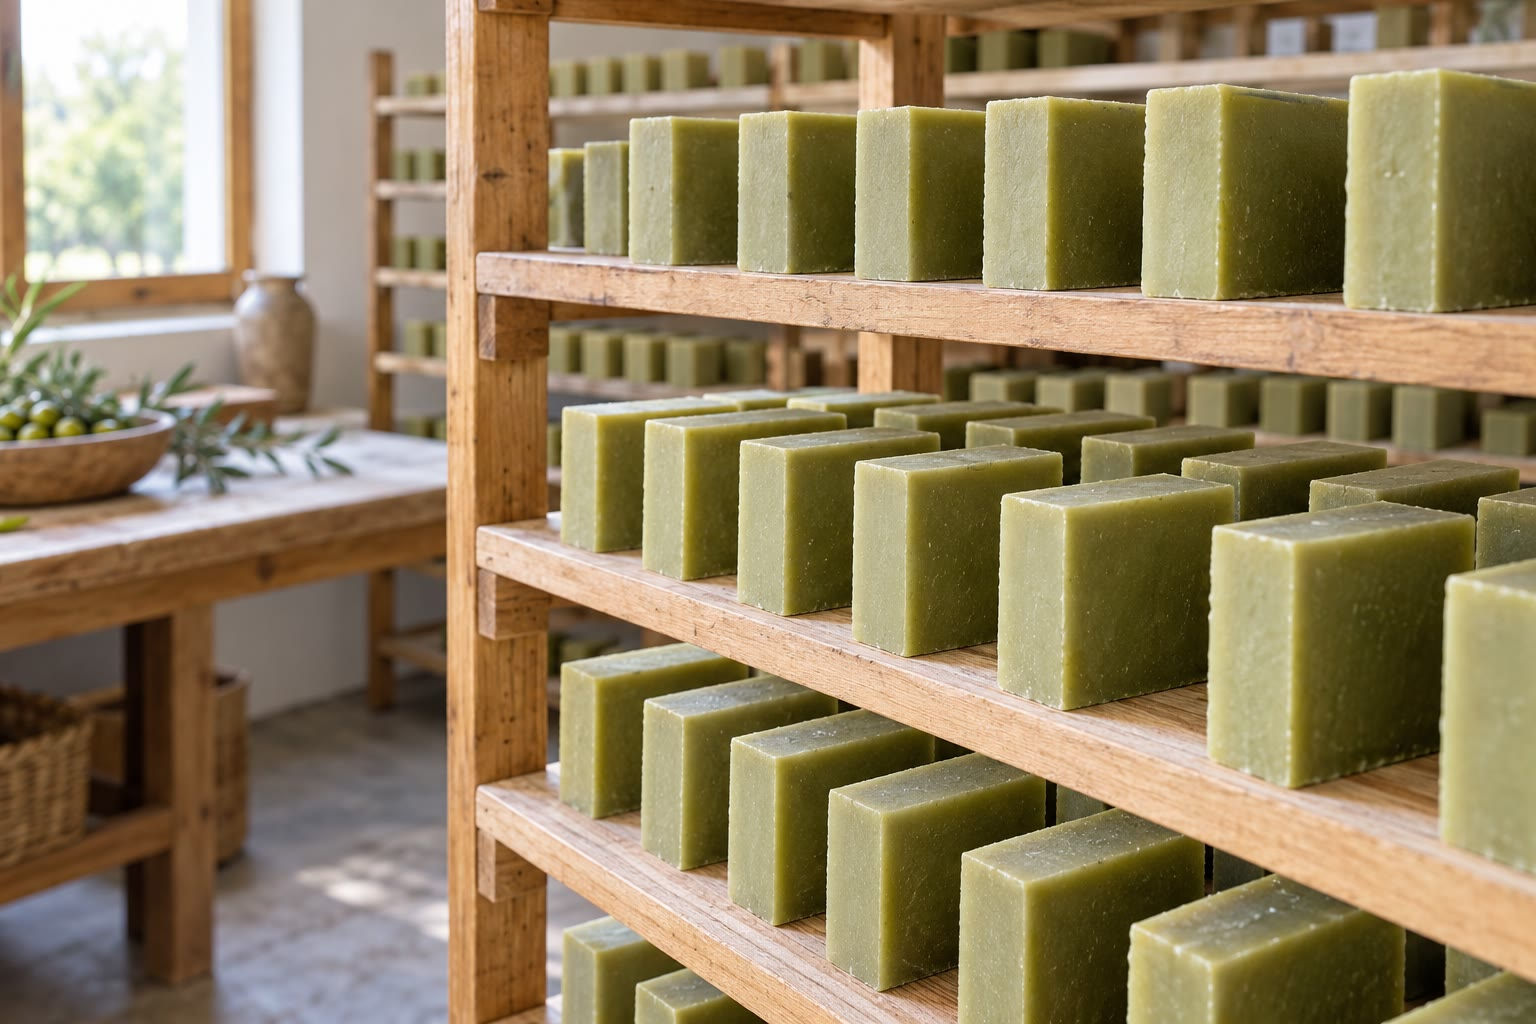
\includegraphics[width=0.58\linewidth]{images/book3/ai/b2-24-soap-bars.jpg}

{\small Blokken olijfoliezeep die drogen op houten rekken. Zeep is het natriumzout van de vetzuren
die vrijkomen wanneer de olie, een ester, met natriumhydroxide gekookt wordt.}
\end{omfigure}

\section{De familie en haar reactiviteit}

\begin{definition}[Carbonzuurderivaten]\label{def:b2:acyl-substitution:derivative}
Een \emph{carbonzuurderivaat}\index{carbonzuurderivaat} is een verbinding \ce{R-CO-Z} waarin
de \ce{OH} van een carbonzuur vervangen is door een andere groep Z. De \emph{acylgroep}\index{acylgroep}
$\mathrm{R{-}CO{-}}$ hebben ze allemaal gemeen. In een \emph{acylchloride}\index{acylchloride}
is Z gelijk aan Cl; in een \emph{zuuranhydride}\index{zuuranhydride} is Z gelijk aan $\mathrm{O{-}CO{-}R'}$: twee acylgroepen
delen één zuurstofatoom; in een ester is Z gelijk aan $\mathrm{OR'}$, in een amide aan $\mathrm{NR'_2}$.
\end{definition}

\begin{proposition}[Reactiviteitsschaal]\label{prop:b2:acyl-substitution:reactivity}
Tegenover nucleofielen reageren de derivaten in de volgorde \omterm{def:b2:acyl-substitution:derivative}{acylchloride} $>$ anhydride $>$ ester
$\approx$ zuur $>$ amide.
\end{proposition}

\begin{proof}[Redenering]
Twee effecten tellen op. De vertrekkende groep \ce{Z-} vertrekt des te gemakkelijker naarmate ze een zwakkere base is:
\ce{Cl-} (geconjugeerd zuur \ce{HCl}, $\mathrm pK_a$ ongeveer $-7$) veel beter dan een carboxylaat
($\mathrm pK_a$ ongeveer 5), een alkoxide (ongeveer 16) of een amide-ion (ongeveer 35). En de groep Z geeft
elektronendichtheid aan de carbonylgroep door mesomere donatie van zijn vrije elektronenpaar, wat het carbonylkoolstofatoom
minder elektrofiel maakt: zwak bij Cl, het sterkst bij stikstof. Het amide is zowel het zwakste
elektrofiel als de slechtste vertrekkende groep.
% ledger: pka:ethanoic, pka:ethanol
\end{proof}

\section{Nucleofiele acylsubstitutie}

\begin{definition}[Nucleofiele acylsubstitutie]\label{def:b2:acyl-substitution:nas}
Een \emph{nucleofiele acylsubstitutie}\index{nucleofiele acylsubstitutie} vervangt de groep Z
van een acylverbinding door een nucleofiel. Ze verloopt via additie van het nucleofiel aan het carbonylkoolstofatoom,
wat een \emph{tetraëdrisch intermediair}\index{tetraedrisch intermediair@tetraëdrisch intermediair} geeft, gevolgd door
eliminatie van de vertrekkende groep, die de binding \ce{C=O} herstelt.
\end{definition}

\begin{proposition}[Additie--eliminatie]\label{prop:b2:acyl-substitution:addition-elimination}
Acylsubstitutie verloopt via een \omterm{def:b2:acyl-substitution:nas}{tetraëdrisch intermediair}; ze wordt in base versneld door een sterker
nucleofiel en in zuur door activering van de carbonylgroep.
\end{proposition}

\begin{proof}[Redenering]
Het carbonylkoolstofatoom, vlak en elektrofiel, neemt het nucleofiel op van boven of onder zijn
vlak, zoals bij de addities van \cref{ch:b2:amines}; met een groep Z die kan vertrekken, stoot het intermediair
die uit in plaats van geprotoneerd te worden. In base is het nucleofiel een anion (\ce{HO-},
\ce{RO-}); in zuur wordt het carbonylzuurstofatoom geprotoneerd en volstaat een neutraal nucleofiel (water, een alcohol).
Esters die in het alcoholdeel met \ce{^{18}O} gemerkt zijn, geven bij hydrolyse gemerkte alcohol
en ongemerkt zuur: de verbroken binding is de binding acyl--zuurstof, zoals het mechanisme vereist.
\end{proof}

\begin{omfigure}
\setchemfig{atom sep=1.7em}
\schemestart
\chemfig{R-C(=[2]O)-OR'} \+ \chemfig{HO^{-}}
\arrow{->[additie]}
\chemfig{R-C(-[2]O^{-})(-[6]OH)-OR'}
\arrow{->[eliminatie]}[,1.3]
\chemfig{R-C(=[2]O)-OH} \+ \chemfig{^{-}OR'}
\schemestop

\medskip
\schemestart
\chemfig{R-C(=[2]O)-OH} \+ \chemfig{^{-}OR'}
\arrow{->[protonoverdracht]}
\chemfig{R-C(=[2]O)-O^{-}} \+ \chemfig{HOR'}
\schemestop
\par\vspace{6pt}

{\small \omterm{def:b2:acyl-substitution:saponification}{Verzeping} van een ester. Hydroxide addeert aan het carbonylkoolstofatoom en geeft het \omterm{def:b2:acyl-substitution:nas}{tetraëdrische
intermediair}; het alkoxide vertrekt en de binding \ce{C=O} vormt zich opnieuw; het alkoxide, een sterke base, neemt daarna
het proton van het zuur op. Deze laatste stap maakt de reactie volledig.}
\end{omfigure}

\begin{method}[Een acylsubstitutie tekenen]\label{met:b2:acyl-substitution:nas-mechanism}
\begin{enumerate}
  \item In base: het anionische nucleofiel addeert aan het carbonylkoolstofatoom; de negatieve lading gaat naar
        zuurstof; de binding \ce{C=O} vormt zich opnieuw en Z vertrekt; sluit af met een eventuele zuur-basestap.
  \item In zuur: protoneer het carbonylzuurstofatoom; het neutrale nucleofiel addeert; draag een proton over
        naar de vertrekkende groep; die vertrekt als neutraal molecuul; deprotoneer de carbonylgroep.
  \item Tel de stappen: elk intermediair is ofwel tetraëdrisch, ofwel een carbonylverbinding.
\end{enumerate}
\end{method}

\section{Esters}

\begin{definition}[Verestering]\label{def:b2:acyl-substitution:esterification}
Een \emph{verestering}\index{verestering} vormt een ester uit een carbonzuur (of een reactiever
derivaat) en een alcohol. De rechtstreekse reactie van een zuur met een alcohol, gekatalyseerd door een
sterk zuur, is de fischerverestering.
\end{definition}

\begin{proposition}[Fischerverestering]\label{prop:b2:acyl-substitution:fischer}
De fischerverestering is een traag evenwicht, met een constante rond 4 voor primaire alcoholen; ze
wordt vooruitgedreven door een overmaat van één reagens of door water te verwijderen naarmate het ontstaat.
\end{proposition}

\begin{proof}[Redenering]
Equimolair ethanol en ethaanzuur stoppen wanneer twee derde van het zuur veresterd is: $K =
(2/3)^2/(1/3)^2 = 4$. Met $Q < K$, in stand gehouden door een overmaat alcohol of door water af te destilleren
(de Dean--Stark-opvanger uit het deel van jaar~1), gaat de reactie verder
(\cref{ch:b2:equilibrium-shifts}). De zes stappen van het mechanisme zijn die van \cref{met:b2:acyl-substitution:nas-mechanism}
in zuur, allemaal omkeerbaar.
% ledger: ester:berthelot
\end{proof}

\begin{definition}[Verzeping]\label{def:b2:acyl-substitution:saponification}
Een \emph{verzeping}\index{verzeping} is de hydrolyse van een ester door een hydroxide, die
het carboxylaatzout en de alcohol geeft.
\end{definition}

\begin{proposition}[Verzeping is volledig]\label{prop:b2:acyl-substitution:saponification}
\omterm{def:b2:acyl-substitution:saponification}{Verzeping} verloopt volledig: haar laatste stap, de protonoverdracht van het carbonzuur naar
het alkoxide, heeft een evenwichtsconstante van de orde $10^{11}$.
\end{proposition}

\begin{proof}
Voor $\mathrm{RCOOH + R'O^- \to RCOO^- + R'OH}$ geldt
\[
  K = \frac{K_a(\ce{RCOOH})}{K_a(\mathrm{R'OH})} = 10^{\mathrm pK_a(\mathrm{R'OH}) - \mathrm pK_a(\ce{RCOOH})} ;
\]
met ethaanzuur (4.76) en ethanol (15.93) is $K = 10^{11.2}$. Het carboxylaat, een zwak elektrofiel, wordt niet aangevallen door de alcohol: de totale
reactie keert niet terug.
% ledger: pka:ethanoic, pka:ethanol
\end{proof}

\begin{omfigure}
\setchemfig{atom sep=1.7em}
\schemestart
\chemfig{CH_2(-[0]O-CO-R)-[6]CH(-[0]O-CO-R)-[6]CH_2-[0]O-CO-R}
\+ \chemfig{3\,NaOH}
\arrow{->[verhitten]}
\chemfig{CH_2(-[0]OH)-[6]CH(-[0]OH)-[6]CH_2-[0]OH}
\+ \chemfig{3\,R-COO^{-}\,Na^{+}}
\schemestop
\par\vspace{6pt}

{\small \omterm{def:b2:acyl-substitution:saponification}{Verzeping} van een triglyceride: de drie esterbindingen worden doorgeknipt, wat glycerol en
drie moleculen natriumcarboxylaat geeft, de zeep (R een lange keten, \ce{C17H33} voor het oleaat van
olijfolie).}
\end{omfigure}

\begin{definition}[Omestering]\label{def:b2:acyl-substitution:transesterification}
Een \emph{omestering}\index{omestering} wisselt het alcoholdeel van een ester uit,
$\mathrm{RCOOR' + R''OH \rightleftharpoons RCOOR'' + R'OH}$, onder zure of basische katalyse.
\end{definition}

\begin{definition}[Lactonen en lactamen]\label{def:b2:acyl-substitution:lactone}
Een \emph{lacton}\index{lacton} is een cyclische ester, gevormd door interne \omterm{def:b2:acyl-substitution:esterification}{verestering} van een
hydroxyzuur; een \emph{lactam}\index{lactam} is een cyclisch amide.
\end{definition}

\section{Geactiveerde derivaten}

De reactiviteitsschaal afdalen is gemakkelijk: een \omterm{def:b2:acyl-substitution:derivative}{acylchloride} geeft met het juiste nucleofiel een anhydride, een ester of een
amide, vaak bij kamertemperatuur. Klimmen vraagt activering: een
carbonzuur wordt met thionylchloride omgezet in zijn chloride,
\[
  \ce{RCOOH + SOCl2 -> RCOCl + SO2 + HCl} ,
\]
waarvan de bijproducten gassen zijn. Het \omterm{def:b2:acyl-substitution:derivative}{acylchloride} reageert daarna met een alcohol of een amine; een base
(pyridine, triethylamine, of een tweede equivalent van het amine) vangt het gevormde \ce{HCl} weg, dat
anders het amine zou protoneren.

\begin{method}[Langs de derivaten bewegen]\label{met:b2:acyl-substitution:ladder}
\begin{enumerate}
  \item Omlaag op de schaal (chloride $\to$ anhydride $\to$ ester, zuur $\to$ amide): behandel met het
        nucleofiel, met een base om het vrijgekomen zuur op te nemen.
  \item Omhoog op de schaal: zet het zuur eerst om in het chloride (\ce{SOCl2}); een ester of amide wordt
        eerst tot het zuur gehydrolyseerd.
  \item Tussen een zuur en een ester: fischerverestering (evenwicht) of \omterm{def:b2:acyl-substitution:saponification}{verzeping}
        (volledig) gevolgd door aanzuren.
\end{enumerate}
\end{method}

\begin{omfigure}
\begin{tikzpicture}[font=\small, >={Stealth}]
  \foreach \y/\n in {4/{acylchloride \ce{RCOCl}}, 3/{anhydride \ce{(RCO)2O}}, 2/{ester $\mathrm{RCOOR'}$ \quad zuur \ce{RCOOH}}, 1/{amide $\mathrm{RCONR'_2}$}} {
    \node[cyclenode, minimum width=5.2cm] at (0,\y*1.1) {\n};
  }
  \draw[->, thick, omDef] (-3.1,4.3) -- (-3.1,1.1) node[midway, left, align=right, font=\scriptsize] {makkelijk:\\ nucleofiel\\ + base};
  \draw[->, thick, omThm] (3.1,2.2) -- (3.1,4.4) node[midway, right, align=left, font=\scriptsize] {bergop:\\ via het zuur\\ en \ce{SOCl2}};
  \node[font=\scriptsize, anchor=south] at (0,4.85) {reactiever};
  \node[font=\scriptsize, anchor=north] at (0,0.55) {minder reactief};
\end{tikzpicture}

{\small De reactiviteitsladder van de carbonzuurderivaten. Elk derivaat kan door een nucleofiel omgezet worden in
een derivaat eronder; klimmen gaat via het zuur en zijn chloride.}
\end{omfigure}

\section{Organometaalverbindingen en hydriden}

\begin{proposition}[Twee grignardaddities]\label{prop:b2:acyl-substitution:grignard-ester}
Een ester die met een overmaat organomagnesiumverbinding behandeld wordt, geeft een tertiaire alcohol met twee
identieke groepen uit het reagens.
\end{proposition}

\begin{proof}[Redenering]
De eerste additie geeft een \omterm{def:b2:acyl-substitution:nas}{tetraëdrisch intermediair} dat het alkoxide uitstoot: een keton. Een keton
is elektrofieler dan een ester (geen mesomere donatie van een groep $\mathrm{OR'}$) en reageert met
het reagens sneller dan de resterende ester; de tweede additie, aan het keton, geeft het alkoxide
van een tertiaire alcohol, dat bij de zure opwerking geprotoneerd wordt. De reactie kan niet bij het keton gestopt worden.
\end{proof}

\begin{proposition}[Reducties met hydriden]\label{prop:b2:acyl-substitution:hydrides}
Lithiumaluminiumhydride reduceert esters en zuren tot primaire alcoholen, en amiden tot aminen;
natriumboorhydride reduceert aldehyden en ketonen, maar geen esters, zuren of amiden. Een omvangrijk aluminiumhydride
(DIBAL-H) reduceert bij \qty{-78}{\degreeCelsius} een ester tot het aldehyde.
\end{proposition}

\begin{proof}[Redenering]
\ce{LiAlH4} is een sterke hydridedonor: net als het grignardreagens addeert het twee keer aan een ester (via
het aldehyde). Boorhydride is te zwak voor de minder elektrofiele carbonylgroep van een ester. Met DIBAL-H bij
lage temperatuur stoot het \omterm{def:b2:acyl-substitution:nas}{tetraëdrische intermediair}, vastgehouden door aluminium, het alkoxide pas uit bij
de waterige opwerking, wanneer er geen hydride meer over is: het aldehyde blijft over. In een amide wordt het zuurstofatoom,
gebonden aan aluminium, geëlimineerd in plaats van het stikstofatoom, wat een iminiumion achterlaat dat het hydride
tot het amine reduceert.
\end{proof}

\begin{history}[Chevreul en de vetten]
\begin{minipage}[t]{0.22\linewidth}
\vspace{0pt}
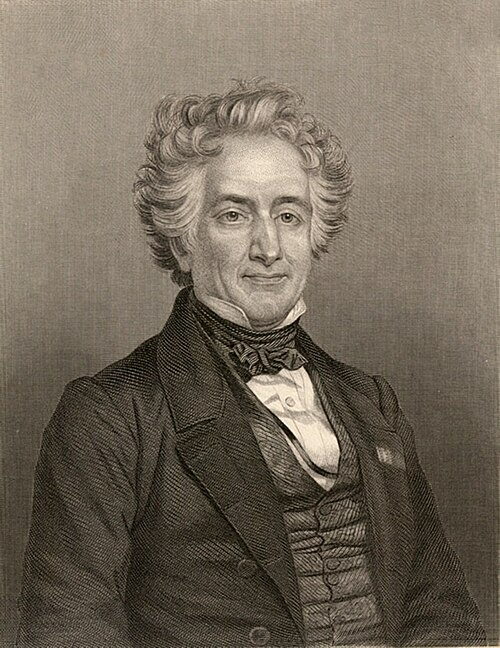
\includegraphics[width=\linewidth]{images/book3/chevreul.jpg}
\end{minipage}\hfill
\begin{minipage}[t]{0.74\linewidth}
\vspace{0pt}
Michel Eugène Chevreul toonde in een studie die in 1823 verscheen aan dat vetten verbindingen zijn van glycerol
met vetzuren, die hij isoleerde en een naam gaf (stearinezuur, oliezuur, boterzuur), en dat
\omterm{def:b2:acyl-substitution:saponification}{verzeping} ze in die twee delen splitst. Zijn werk maakte van het zepen- en kaarsenmaken
scheikunde; hij werd 102 jaar oud. (Portret door Nicolas Eustache Maurin, publiek domein, Wikimedia
Commons.)
\end{minipage}
\end{history}

\begin{safety}{\ghs[5mm]{GHS02}\,\ghs[5mm]{GHS05}\,\ghs[5mm]{GHS06}}
Thionylchloride en \omterm{def:b2:acyl-substitution:derivative}{acylchloriden} reageren heftig met water en maken corrosieve gassen vrij; ze
worden droog gehanteerd, in een zuurkast. Lithiumaluminiumhydride ontbrandt bij contact met water; de
overmaat wordt op het einde voorzichtig vernietigd. Geconcentreerd natriumhydroxide is corrosief voor huid en
ogen. Methanol is giftig en ontvlambaar.
% ledger: ghs:SOCl2, ghs:ethanoyl-chloride, ghs:LiAlH4, ghs:NaOH, ghs:methanol
\end{safety}

\section{Oefeningen}

\begin{exercise}[$\star$]\label{exo:b2:acyl-substitution:1}
Rangschik naar reactiviteit tegenover water: ethylethanoaat, ethanoylchloride, ethaanamide,
ethaanzuuranhydride.
\end{exercise}

\begin{exercise}[$\star$]\label{exo:b2:acyl-substitution:2}
Geef de producten van ethanoylchloride met: water; ethanol; ammoniak (2 equivalenten);
natriumethanoaat; dimethylamine met triethylamine.
\end{exercise}

\begin{exercise}[$\star$]\label{exo:b2:acyl-substitution:3}
Schrijf de \omterm{def:b2:acyl-substitution:saponification}{verzeping} van methylbenzoaat door natriumhydroxide op en bereken de massa natriumhydroxide
die nodig is voor \qty{13.6}{g} van de ester.
\end{exercise}

\begin{exercise}[$\star$]\label{exo:b2:acyl-substitution:4}
Teken het \omterm{def:b2:acyl-substitution:lactone}{lacton} dat 4-hydroxybutaanzuur vormt en geef de grootte van zijn ring.
\end{exercise}

\begin{exercise}[$\star\star$]\label{exo:b2:acyl-substitution:5}
Schrijf het mechanisme op van de reactie van ethylethanoaat met ammoniak.
\end{exercise}

\begin{exercise}[$\star\star$]\label{exo:b2:acyl-substitution:6}
Aspirine wordt gemaakt uit salicylzuur (2-hydroxybenzoëzuur) en ethaanzuuranhydride. Welke groep
van salicylzuur reageert, en wat is het bijproduct?
\end{exercise}

\begin{exercise}[$\star\star$]\label{exo:b2:acyl-substitution:7}
Ethylethanoaat wordt behandeld met een overmaat methylmagnesiumbromide en daarna met verdund zuur. Geef het
product en leg uit waarom het keton niet geïsoleerd kan worden.
\end{exercise}

\begin{exercise}[$\star\star$]\label{exo:b2:acyl-substitution:8}
Geef het product van de reductie van het \omterm{def:b2:acyl-substitution:lactone}{lacton} van oefening 4 door \ce{LiAlH4}.
\end{exercise}

\begin{exercise}[$\star\star$]\label{exo:b2:acyl-substitution:9}
Bereken met $K = 4$ de fractie ethaanzuur die veresterd wordt met één, en daarna met drie
equivalenten ethanol. Welke andere methode drijft de reactie voort?
\end{exercise}

\begin{exercise}[$\star\star\star$]\label{exo:b2:acyl-substitution:10}
Bereid \textit{N},\textit{N}-diethylbenzamide uit benzoëzuur, en leg uit waarom het zuur mengen
met diethylamine en zacht verwarmen in plaats daarvan een zout geeft.
\end{exercise}

\begin{exercise}[$\star\star\star$]\label{exo:b2:acyl-substitution:11}
Het verzepingsgetal van een vet is de massa kaliumhydroxide, in mg, die nodig is om
\qty{1}{g} ervan te verzepen. Bereken het voor trioleïne (\qty{885.4}{g/mol}; KOH \qty{56.11}{g/mol}).
\end{exercise}

\begin{exercise}[$\star\star\star$]\label{exo:b2:acyl-substitution:12}
Een molecuul draagt een ester, een amide en een keton. Welke groep(en) reduceert \ce{NaBH4}, en welke
\ce{LiAlH4}? Wat verkrijg je in elk geval?
\end{exercise}

\section{Probleem: biodiesel uit frituurolie}

\begin{problem}[{Weekendprobleem --- trioleïne en zijn molaire massa, zijn omestering met
methanol en de rol van de base, de nevenreactie met vrije zuren en water, en de opbrengsten per
ton olie}]
\label{pb:b2:acyl-substitution:1}
Beschouw de olie als zuivere trioleïne, het triglyceride van oliezuur (\ce{C17H33COOH}). Molaire massa's
(\unit{g/mol}): C 12.011, H 1.008, O 15.999, Na 22.990. Glycerol is propaan-1,2,3-triol.
% ledger: aw:C, aw:H, aw:O, aw:Na, ghs:methanol, ghs:NaOH

\medskip
\noindent\textbf{Deel I --- Trioleïne.}
\begin{enumerate}
  \item Geef de formule van oliezuur en van glycerol.
  \item Schrijf de formule van trioleïne op en bereken zijn molaire massa.
  \item Hoeveel estergroepen bevat het?
  \item Oliezuur heeft één cis-dubbele binding. Waarom zijn oliën die er rijk aan zijn vloeibaar bij kamertemperatuur?
  \item Wat zou \omterm{def:b2:acyl-substitution:saponification}{verzeping} van trioleïne geven?
  \item Wat is biodiesel, chemisch gezien?
\end{enumerate}

\medskip
\noindent\textbf{Deel II --- \omterm{def:b2:acyl-substitution:transesterification}{Omestering}.}
\begin{enumerate}[resume]
  \item Schrijf de \omterm{def:b2:acyl-substitution:transesterification}{omestering} van trioleïne met methanol op.
  \item Waarom wordt een base (natriummethoxide of -hydroxide) als katalysator gebruikt?
  \item Teken het \omterm{def:b2:acyl-substitution:nas}{tetraëdrische intermediair} van de eerste uitwisseling.
  \item Waarom wordt methanol in overmaat gebruikt (zes equivalenten in plaats van drie)?
  \item Glycerol mengt niet met de methylesters. Waarom helpt dat?
  \item Wordt de katalysator verbruikt in de ideale reactie?
\end{enumerate}

\medskip
\noindent\textbf{Deel III --- Vrije zuren en water.}
\begin{enumerate}[resume]
  \item Gebruikte frituurolie bevat vrij oliezuur. Wat doet dat met de base?
  \item Wat doet water met de methylesters in aanwezigheid van de base?
  \item Waarom is de gevormde zeep hinderlijk?
  \item Hoe kunnen de vrije zuren eerst verwijderd worden, zonder base?
  \item Waarom moet de olie vóór de reactie gedroogd worden?
\end{enumerate}

\medskip
\noindent\textbf{Deel IV --- Per ton olie.}
\begin{enumerate}[resume]
  \item Bereken de hoeveelheid trioleïne in één ton.
  \item Bereken de massa verbruikte methanol.
  \item Bereken de massa gevormd methyloleaat.
  \item Controleer het behoud van massa.
  \item Een olie met 2~\% vrij oliezuur in massa wordt behandeld met natriumhydroxide: bereken de massa
        natriumhydroxide die per ton door het zuur verbruikt wordt.
  \item Bereken de massa glycerol die per ton trioleïne als nevenproduct ontstaat.
\end{enumerate}
\end{problem}
